\chapter{Results}
\label{08_ergebnisse}

The workflow was applied to five study areas in the Global South introduced in Section~\ref{ch:study_area}. This chapter reports the pipeline coverage, changes in manually assessed polygon quality and error composition, geometric changes after refinement, the MLLM outputs, and the supplementary reference-based test in Switzerland. Unless stated otherwise, percentages refer to the latest manual evaluation for each of the 1,256 evaluated buildings. Percentages are rounded to one decimal place.

\section{Processed Dataset and Pipeline Coverage}

\subsection{MLQA Classification and Manual Evaluation Sample}

In total, 2,842 building polygons from the Google Open Buildings dataset were analyzed by the MLQA stage. The mutually exclusive routing classes comprised 1,283 cases classified as \textit{No visible}, 971 as \textit{Partial house}, and 588 as \textit{Full house}. Thus, 1,559 buildings were routed as visible partial- or full-house cases. A SAM-derived polygon was available for 1,518 buildings, a post-processed polygon for 1,352 buildings, and 1,256 buildings were included in the manual evaluation. The evaluated subset contains buildings for which the original and final geometries could be assigned and assessed consistently.

\begin{table}[htbp]
\centering
\caption{MLQA routing classes and manually evaluated subset by study area. The categories \textit{No visible}, \textit{Partial house}, and \textit{Full house} are mutually exclusive and sum to the MLQA input count.}
\label{tab:mlqa_overview}
\begin{tabular}{lrrrrr}
\toprule
Country & MLQA input & No visible & Partial house & Full house & Evaluated \\
\midrule
Liberia    & 616 & 111 & 324 & 181 & 380 \\
Mexico     & 500 & 167 & 224 & 109 & 261 \\
Mozambique & 600 & 424 & 122 & 54  & 167 \\
Nepal      & 626 & 359 & 198 & 69  & 192 \\
Niger      & 500 & 222 & 103 & 175 & 256 \\
\midrule
\textbf{Total} & \textbf{2,842} & \textbf{1,283} & \textbf{971} & \textbf{588} & \textbf{1,256} \\
\bottomrule
\end{tabular}
\end{table}

Cases classified as \textit{No visible} indicate that no corresponding visible building could be identified in the selected aerial or satellite imagery. The distinction between \textit{Partial house} and \textit{Full house}, and the resulting routing decision, are described in Section~\ref{sec:decision_logic_routing}.

\subsection{Pipeline Output Availability}

Table~\ref{tab:pipeline_dropoff} reports the number of unique buildings with outputs at each processing stage. The largest reduction occurred between MLQA input and available SAM output. Once a SAM-derived polygon was available, post-processed outputs were stored for 82.6--97.4\% of cases, depending on the study area. The manual evaluation was restricted to the comparable final subset.

\begin{table}[htbp]
\centering
\caption{Pipeline coverage by study area, showing unique buildings analyzed by MLQA, buildings with a SAM-derived output, buildings with a post-processed output, and manually evaluated buildings.}
\label{tab:pipeline_dropoff}
\begin{tabular}{lrrrrr}
\toprule
Country & MLQA input & SAM output & Post-processed & Evaluated & Post/SAM (\%) \\
\midrule
Liberia    & 616 & 483 & 399 & 380 & 82.6 \\
Mexico     & 500 & 331 & 291 & 261 & 87.9 \\
Mozambique & 600 & 176 & 169 & 167 & 96.0 \\
Nepal      & 626 & 263 & 235 & 192 & 89.4 \\
Niger      & 500 & 265 & 258 & 256 & 97.4 \\
\midrule
\textbf{Total} & \textbf{2,842} & \textbf{1,518} & \textbf{1,352} & \textbf{1,256} & \textbf{89.1} \\
\bottomrule
\end{tabular}
\end{table}

\section{Overall Quality Improvement}

\subsection{Transition from Original to Post-processed Quality}

Figure~\ref{fig:transition_heatmap} shows the transition between the original and post-processed manual ratings. Among the 581 buildings originally rated \textit{bad}, 292 received a final rating of \textit{perfect} and 153 a final rating of \textit{good}; 67 remained \textit{bad}. Among the 656 buildings originally rated \textit{ok}, 382 received a final rating of \textit{perfect} and 134 a rating of \textit{good}. Of the 19 originally \textit{good} buildings, 10 received a final rating of \textit{perfect}. No original polygon was rated \textit{perfect} in this subset.

\begin{figure}[htbp]
\centering
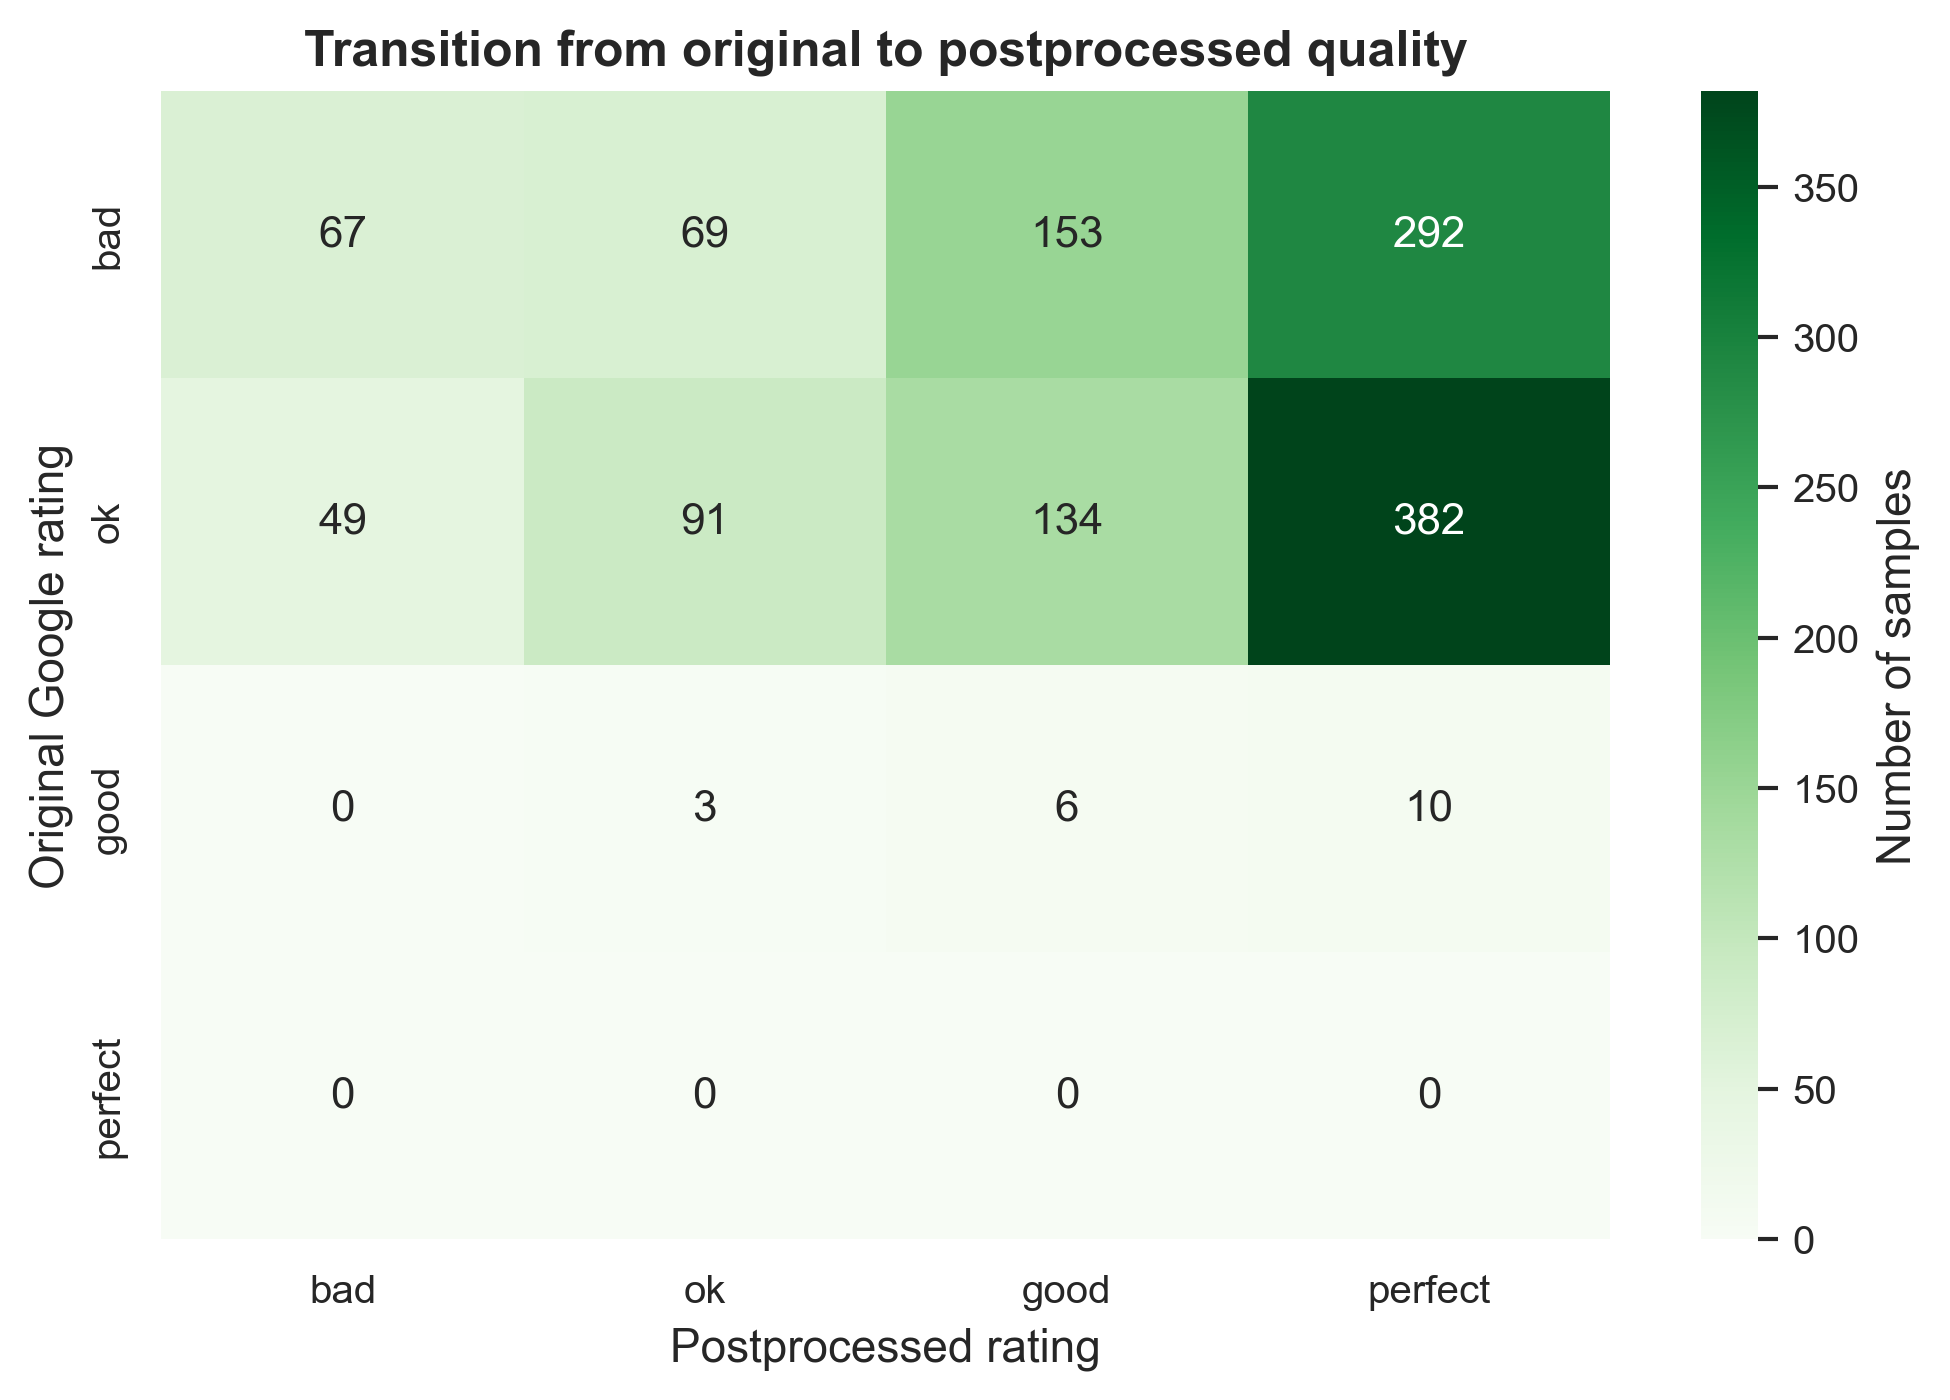
\includegraphics[scale=0.65]{Franzelin_Master/img/02_original_to_post_transition_heatmap.png}
\caption{Transition from original to post-processed manual quality ratings for the evaluated subset (\(n=1,256\)).}
\label{fig:transition_heatmap}
\end{figure}

Overall, the post-processed distribution comprised 116 \textit{bad}, 163 \textit{ok}, 293 \textit{good}, and 684 \textit{perfect} ratings.

\subsection{Improvement Rates by Study Area}

An improvement denotes a higher ordinal manual rating after post-processing, an unchanged case the same rating, and a degradation a lower rating. Across all study areas, 1,040 buildings improved (82.8\%), 164 remained unchanged (13.1\%), and 52 received a lower rating (4.1\%).

Niger had the highest improvement rate at 86.7\% (222/256), followed by Mozambique at 86.2\% (144/167) and Liberia at 86.1\% (327/380). The corresponding unchanged and degraded shares were 9.0\% and 4.3\% in Niger, 10.8\% and 3.0\% in Mozambique, and 12.6\% and 1.3\% in Liberia. Mexico improved in 77.0\% of cases (201/261), with 17.2\% unchanged and 5.7\% degraded. Nepal had an improvement rate of 76.0\% (146/192), with 15.6\% unchanged and 8.3\% degraded.

\begin{figure}[htbp]
\centering
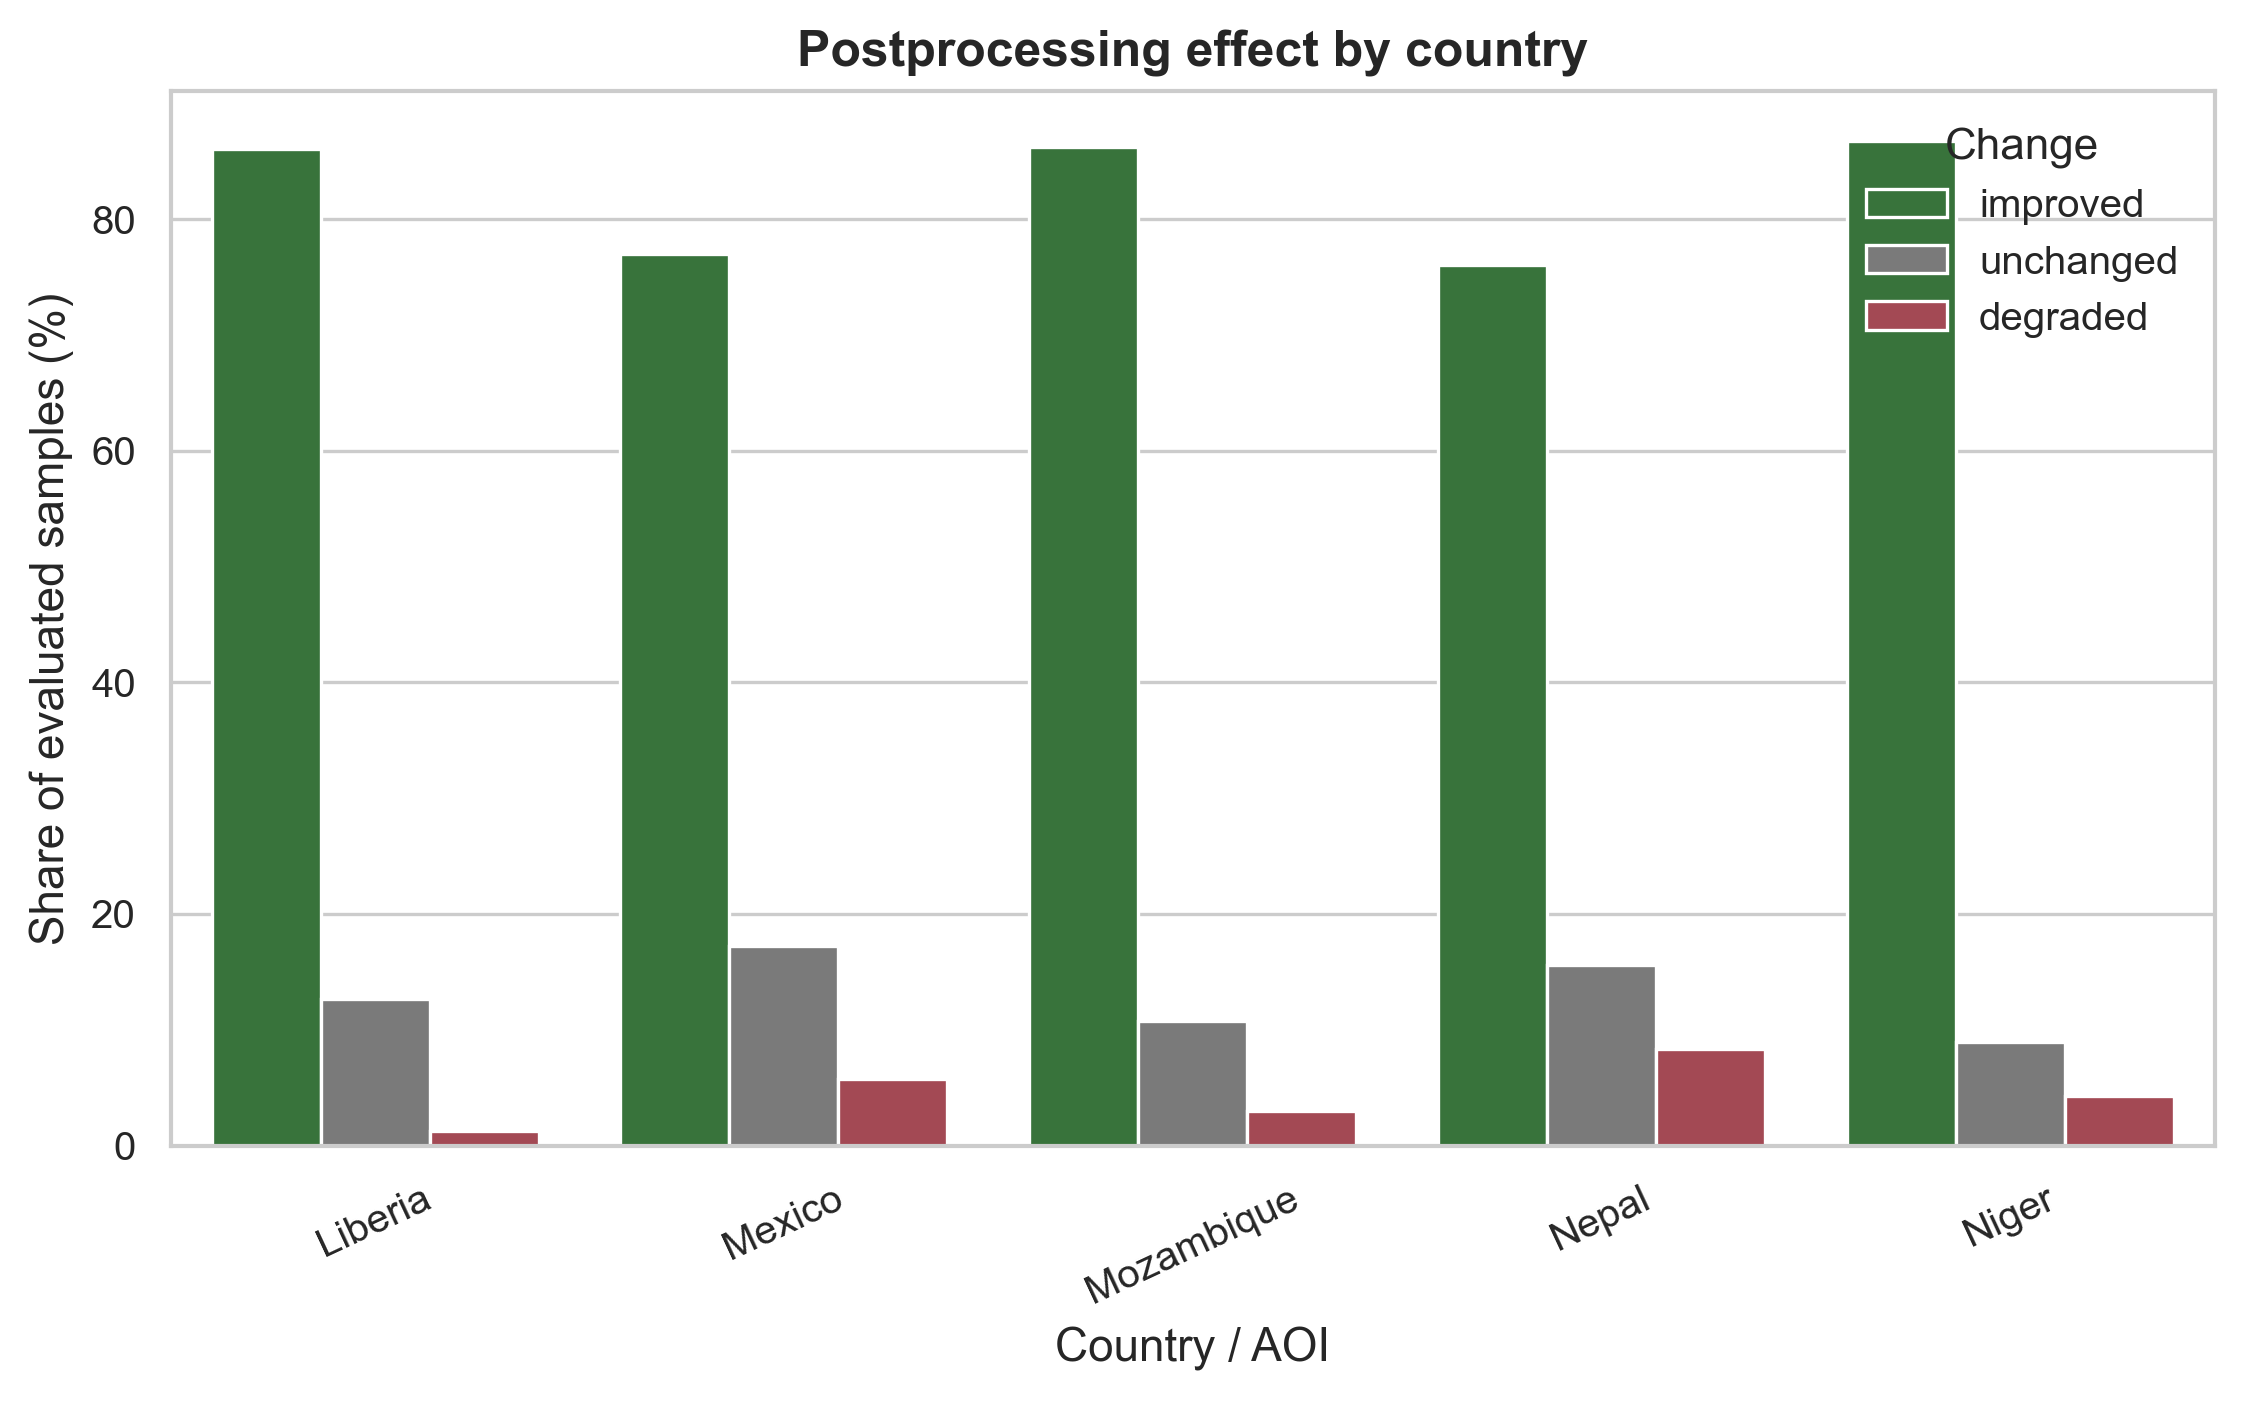
\includegraphics[scale=0.65]{Franzelin_Master/img/02_country_improvement_rates.png}
\caption{Post-processing effect by study area for the manually evaluated subset (\(n=1,256\)). Improved, unchanged, and degraded indicate a higher, equal, or lower ordinal quality rating, respectively.}
\label{fig:country_improvement_rates}
\end{figure}

\subsection{Influence of Google Open Buildings Confidence}

The Google Open Buildings confidence score was compared with the original manual quality rating for all 1,256 evaluated buildings. Pearson's correlation was \(r=0.32\), while Spearman's rank correlation was \(\rho=0.31\). Higher confidence values therefore tended to coincide with higher original quality ratings, although the association was moderate.

\section{Changes in Error Composition}

\subsection{Dominant Errors in Original and Post-processed Geometries}

The error taxonomy is defined in Section~\ref{sec:evaluation_criteria_error_taxonomy}. Because multiple error categories could be assigned to one building, the percentages in Figure~\ref{fig:error_profile_by_location} are not mutually exclusive and can sum to more than 100\%.

\begin{figure}[htbp]
\centering
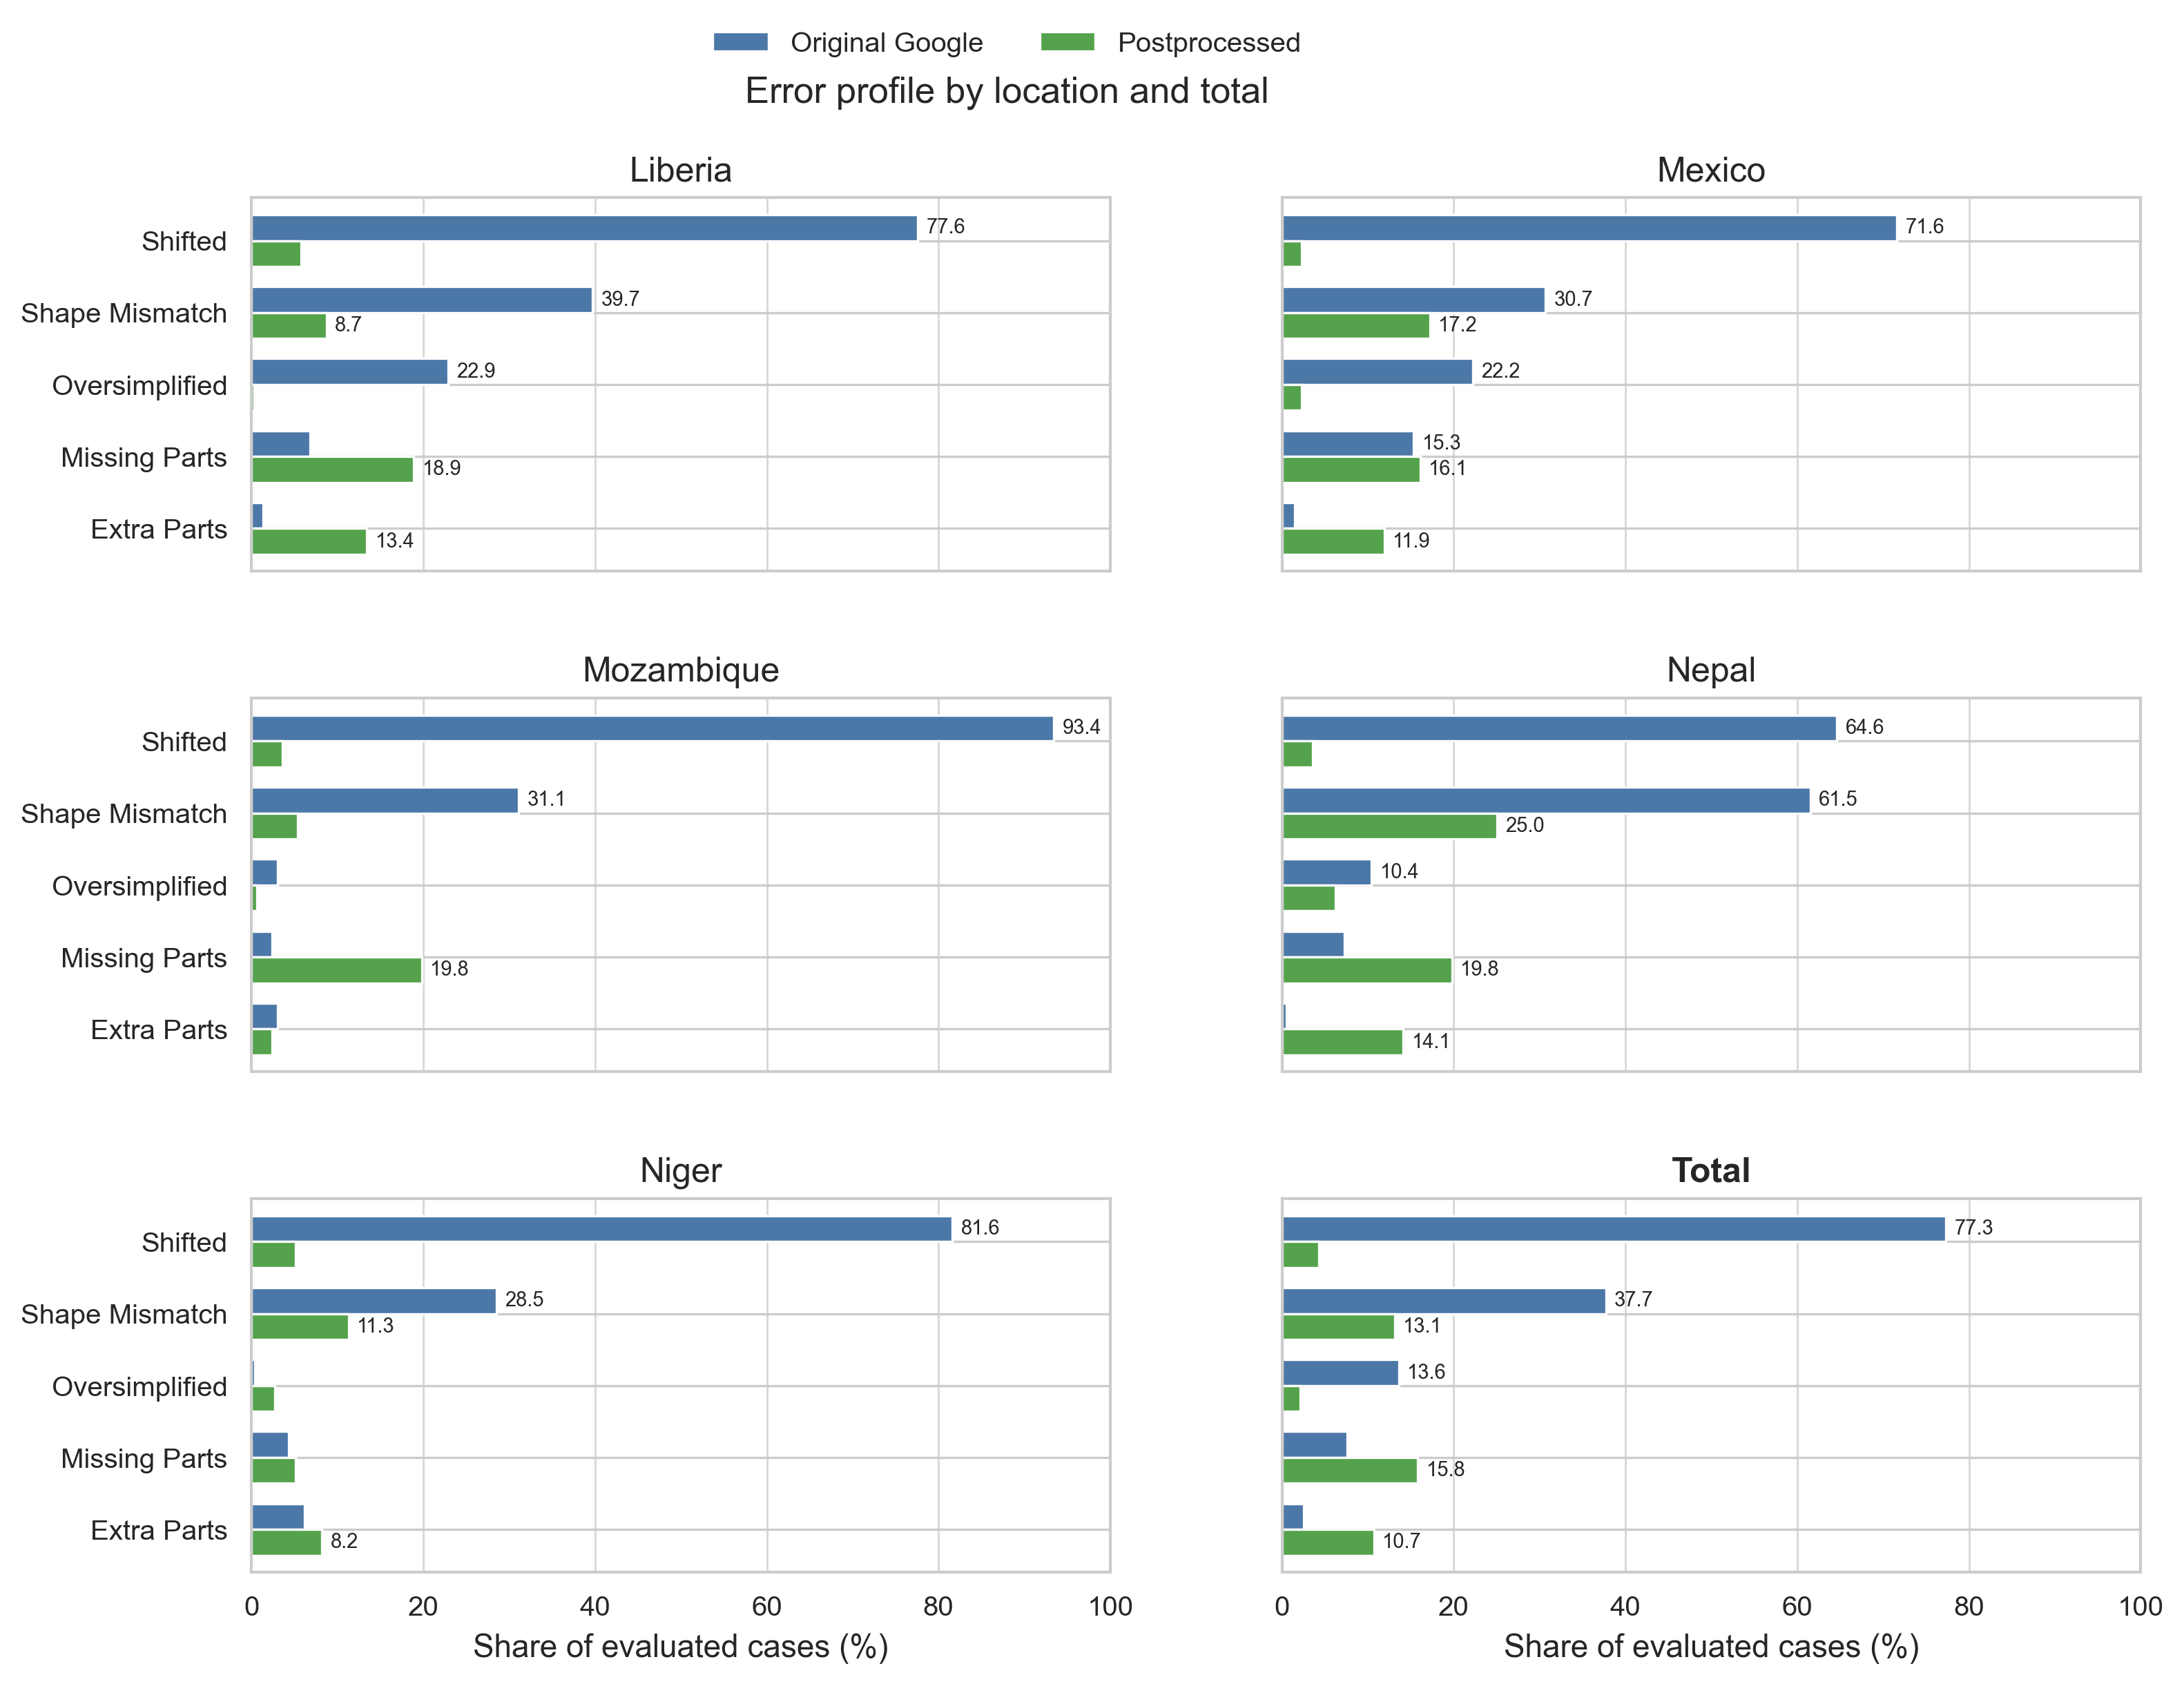
\includegraphics[width=\textwidth]{Franzelin_Master/img/02_error_categories_by_location_total.png}
\caption{Geometry error categories before and after post-processing by study area and for the complete evaluated subset (\(n=1,256\)). Categories are multi-label; percentages are therefore not mutually exclusive.}
\label{fig:error_profile_by_location}
\end{figure}

The most frequent original error was \texttt{SHIFTED}, assigned to 971 buildings (77.3\%). After post-processing, 54 buildings (4.3\%) retained this label. The original shares were highest in Mozambique (93.4\%), Niger (81.6\%), and Liberia (77.6\%); their post-processed shares were 3.6\%, 5.1\%, and 5.8\%, respectively.

The \texttt{SHAPE\_MISMATCH} category decreased from 474 buildings (37.7\%) to 164 (13.1\%). Nepal had the highest original and post-processed shares, at 61.5\% and 25.0\%. \texttt{OVERSIMPLIFIED} decreased from 171 cases (13.6\%) to 27 (2.1\%). In contrast, \texttt{MISSING\_PARTS} increased from 95 cases (7.6\%) to 198 (15.8\%), and \texttt{EXTRA\_PARTS} increased from 31 (2.5\%) to 134 (10.7\%). These increases are examined further in the Discussion.

The manual evaluation recorded a newly introduced post-processing error in 207 of 1,256 buildings (16.5\%). Overall, the largest observed change was the reduction in shifted polygons, while missing and extra parts became more frequent after post-processing.

\subsection{Detected Tree Context and New Post-processing Errors}

Detected tree context was derived from the ratio between the summed detected tree-mask area and the original building area. Cases with no tree mask were classified as \textit{no detected tree}; ratios up to 0.25 as \textit{low}, ratios above 0.25 and up to 1.0 as \textit{medium}, and ratios above 1.0 as \textit{high tree context}. These four classes are mutually exclusive.

Among 530 buildings without a detected tree, 13.4\% received a newly introduced error. Among the 726 buildings with a detected tree, the aggregated rate was 18.7\%. Within the mutually exclusive context classes, the rate ranged from 15.9\% for medium context to 23.0\% for high context. The binary association between detected trees and newly introduced errors was weak (\(\phi=0.07\)).

\begin{table}[htbp]
\centering
\caption{Newly introduced post-processing errors by mutually exclusive detected tree-context class for the evaluated subset (\(n=1,256\)).}
\label{tab:new_errors_tree_context}
\begin{tabular}{lrrrr}
\toprule
Tree context & n & New errors (\%) & Good/perfect (\%) & Missing parts (\%) \\
\midrule
No detected tree & 530 & 13.4 & 83.8 & 8.7 \\
Low              & 189 & 18.0 & 82.5 & 16.9 \\
Medium           & 302 & 15.9 & 75.8 & 21.9 \\
High             & 235 & 23.0 & 63.0 & 23.0 \\
\bottomrule
\end{tabular}
\end{table}

\section{Spatial Shift Analysis}

\subsection{Magnitude and Direction of Positional Corrections}

The shift analysis included the 971 buildings manually labelled \texttt{SHIFTED} in their original state. Centroid displacement was measured from the original polygon to the post-processed polygon using PostGIS geography distances in metres. The vector convention is positive \(dx\) towards the east and positive \(dy\) towards the north. Valid multipart geometries were included through the same centroid calculation.

\begin{figure}[htbp]
\centering
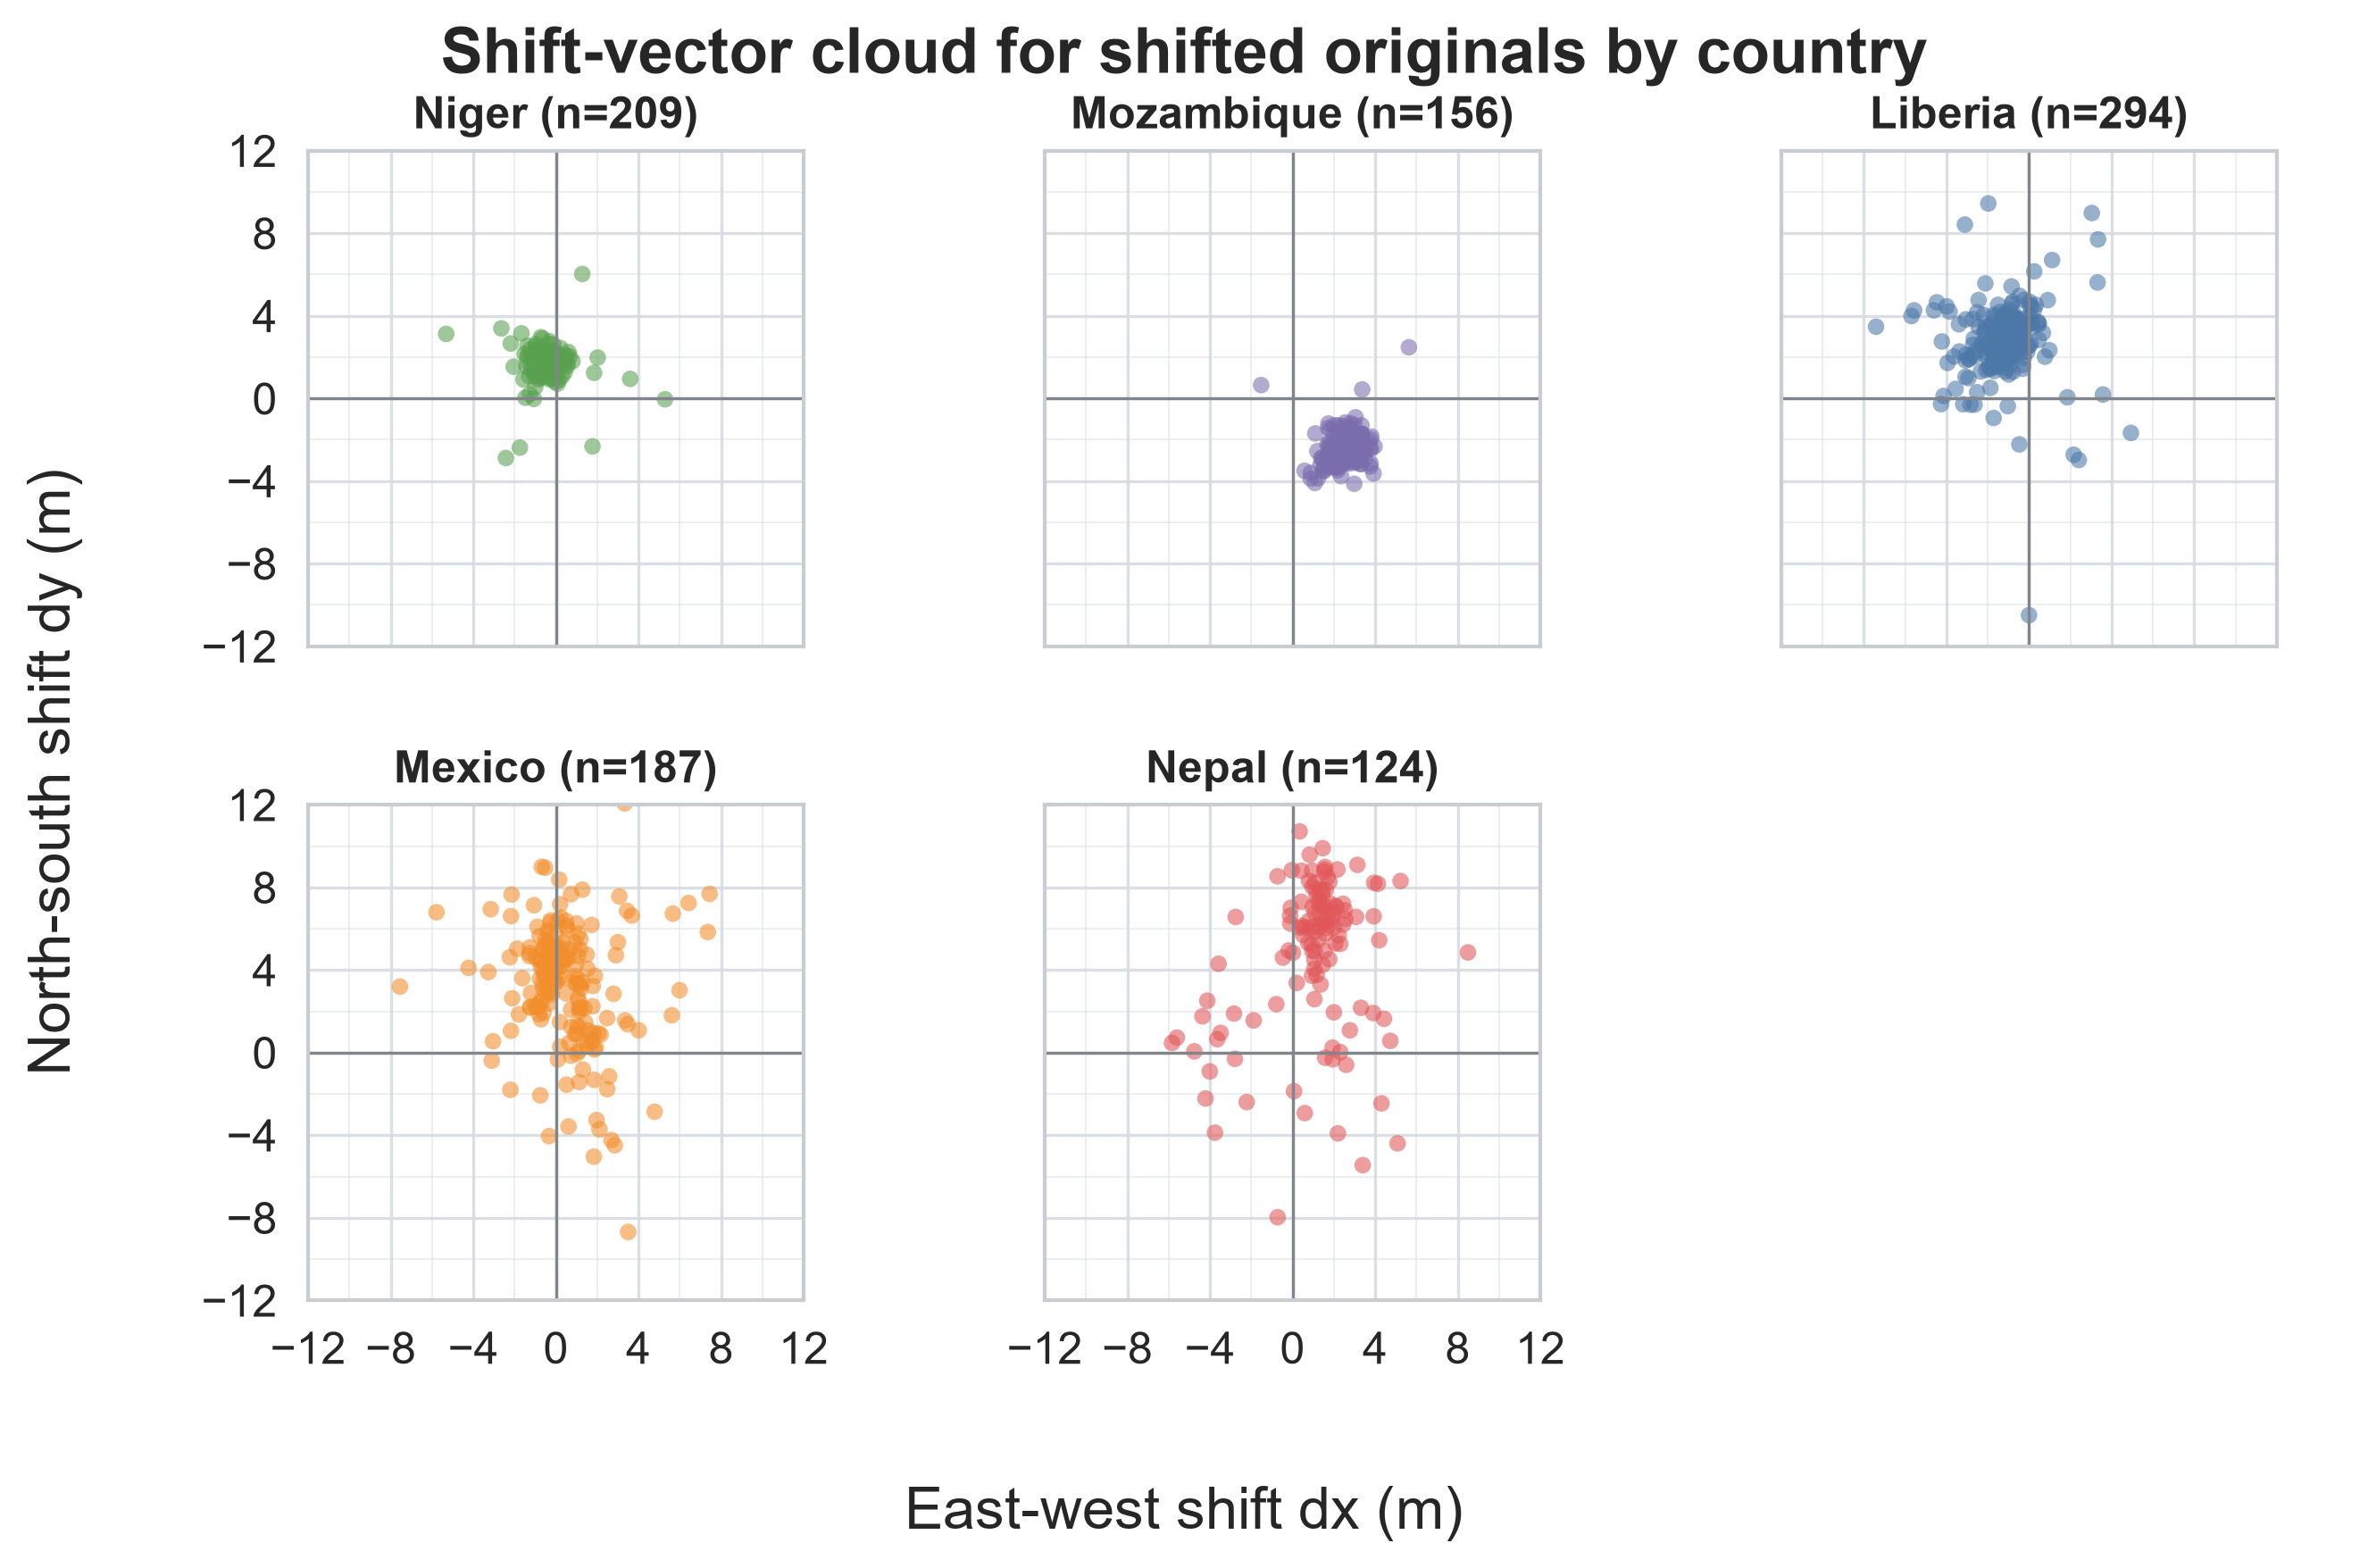
\includegraphics[scale=0.65]{Franzelin_Master/img/04_post_shift_vector_scatter_by_country.png}
\caption{Centroid displacement from the original to the post-processed polygon for buildings originally labelled \texttt{SHIFTED} (\(n=971\)); positive \(dx\) is east and positive \(dy\) is north.}
\label{fig:shift_vectors}
\end{figure}

Nepal showed the largest spread (\(n=124\), \(sd_{dx}=2.61\,\mathrm{m}\), \(sd_{dy}=3.80\,\mathrm{m}\), \(p90=8.88\,\mathrm{m}\)), followed by Mexico (\(n=187\), \(sd_{dx}=1.95\,\mathrm{m}\), \(sd_{dy}=2.94\,\mathrm{m}\), \(p90=7.20\,\mathrm{m}\)). Liberia had \(n=295\), \(sd_{dx}=1.29\,\mathrm{m}\), \(sd_{dy}=1.61\,\mathrm{m}\), and \(p90=4.68\,\mathrm{m}\). Mozambique (\(n=156\)) and Niger (\(n=209\)) showed lower component spreads: \(sd_{dx}=0.79\,\mathrm{m}\) and \(sd_{dy}=0.86\,\mathrm{m}\) in Mozambique, and \(sd_{dx}=0.85\,\mathrm{m}\) and \(sd_{dy}=0.78\,\mathrm{m}\) in Niger.

\section{Geometric Changes After Refinement}

\subsection{Area Preservation}

The signed area change was calculated as \(100(A_{post}/A_{original}-1)\); absolute area change uses the absolute value of this percentage. The scatterplot in Figure~\ref{fig:area_comparison} shows the original and post-processed areas with a 1:1 reference line. For readability, values above the 98th percentile of either axis are omitted from the figure, while the reported percentages use all 1,253 buildings with an available post-processed geometry.

\begin{figure}[htbp]
\centering
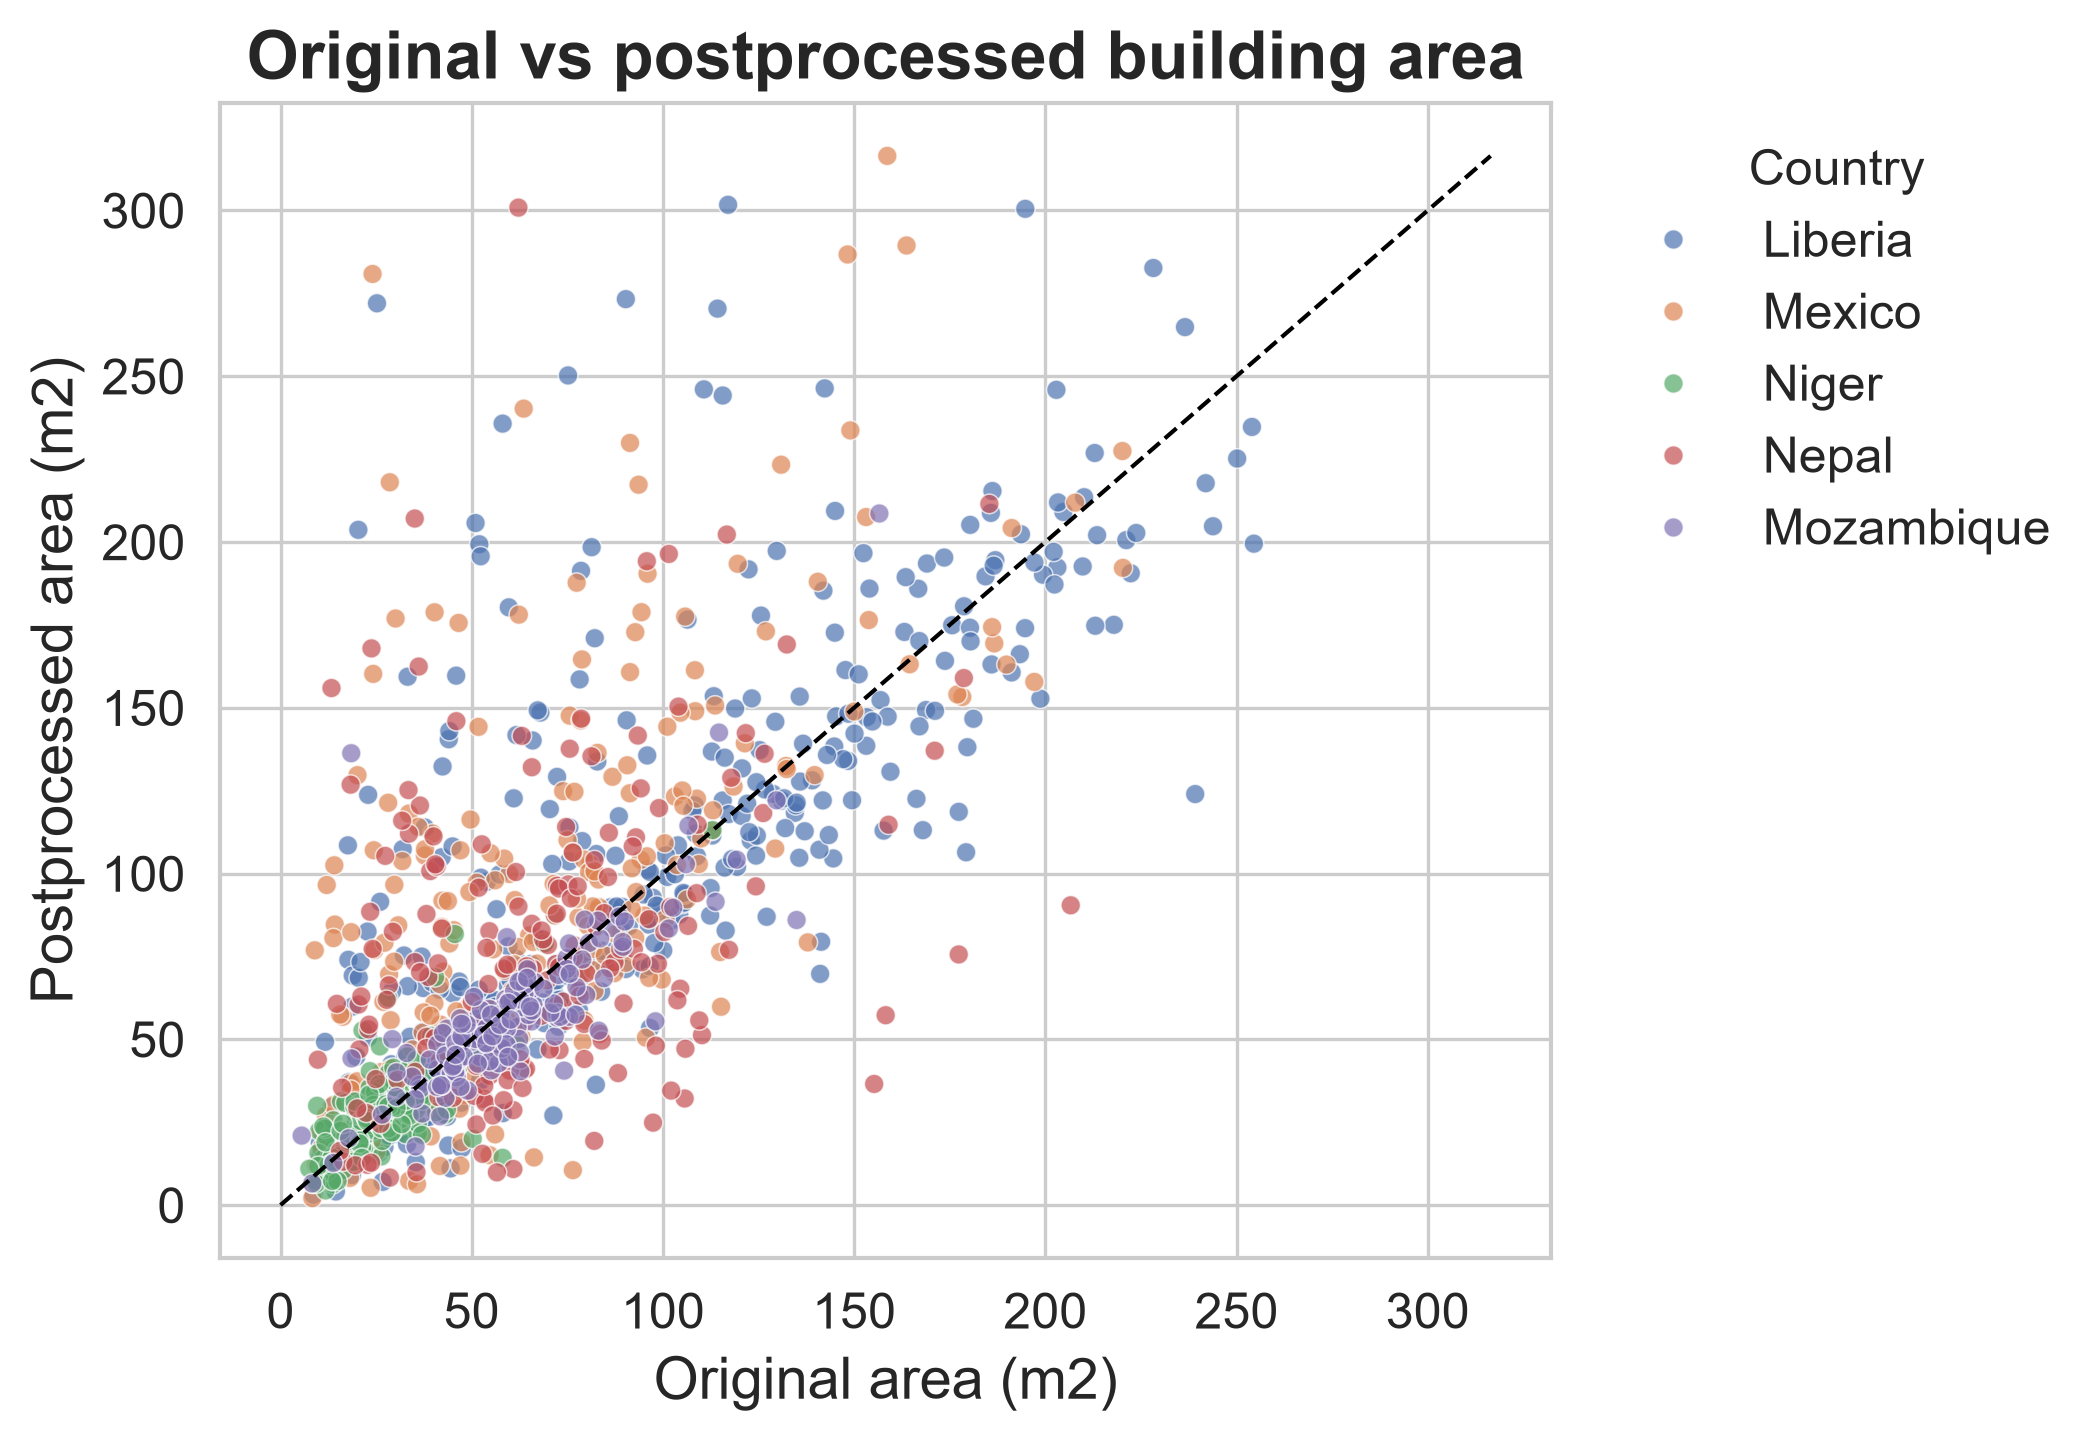
\includegraphics[scale=0.65]{Franzelin_Master/img/03_original_vs_post_area_scatter.png}
\caption{Original and post-processed building areas by study area. The dashed line is the 1:1 reference; values above the 98th percentile of either axis are omitted from the visualization.}
\label{fig:area_comparison}
\end{figure}

In Mozambique, 52.7\% of buildings remained within \(\pm10\%\) of their original area and 2.4\% became more than 50\% larger. The corresponding within-\(\pm10\%\) share was 39.1\% in Niger, 32.1\% in Liberia, 18.8\% in Mexico, and 13.0\% in Nepal. Buildings more than 50\% larger accounted for 20.2\% in Liberia, 31.8\% in Mexico, and 27.1\% in Nepal.

\subsection{Original, SAM-derived, and Post-processed Geometry Complexity}

Table~\ref{tab:stage_geometry_comparison} compares geometry size and vertex counts across stages. Vertex counts were calculated with \texttt{ST\_NPoints} on valid geometries and therefore include all rings, multipart components, and ring-closing coordinates. The three post-processed geometries unavailable for this calculation were all Liberia cases without a stored regularized geometry, resulting in \(n=1,253\) for the final stage.

\begin{table}[htbp]
\centering
\caption{Geometry characteristics of the original, SAM-derived, and post-processed polygons. Vertex counts include all coordinate points returned by \texttt{ST\_NPoints}.}
\label{tab:stage_geometry_comparison}
\begin{tabular}{lrrrr}
\toprule
Stage & n & Mean area (m$^2$) & Mean vertices & Median vertices \\
\midrule
Original Google & 1,256 & 73.02 & 5.27  & 5 \\
SAM-derived     & 1,256 & 77.65 & 40.81 & 39 \\
Post-processed  & 1,253 & 84.64 & 13.45 & 7 \\
\bottomrule
\end{tabular}
\end{table}

The SAM-derived polygons had the highest vertex counts. Post-processing reduced the mean and median vertex counts relative to the SAM-derived geometries, while the final counts remained above those of the original polygons.

\subsection{Full-house and Partial-house Cases}

Within the evaluated subset, 530 \textit{Full house} cases reached a \textit{good} or \textit{perfect} final rating in 79.6\% of cases and had a median absolute area change of 13.5\%. The 723 evaluated \textit{Partial house} cases reached these ratings in 76.3\% of cases and had a median absolute area change of 24.8\%.

\section{Building-to-Surrounding Contrast}

The image-based analysis described in Section~\ref{sec:building_surrounding_contrast} included all 684 buildings with a final rating of \textit{perfect}. Table~\ref{tab:building_surrounding_contrast} reports the median absolute Weber contrast after sRGB linearization and the median Euclidean difference between the building and surrounding texture descriptors.

\begin{table}[htbp]
\centering
\caption{Median building-to-surrounding metrics for all post-processed polygons rated \textit{perfect} (\(n=684\)). Contrast is the absolute linear Weber contrast; texture difference is the Euclidean distance between the building and surrounding texture descriptors.}
\label{tab:building_surrounding_contrast}
\begin{tabular}{lrrr}
\toprule
Country & n & Median Weber contrast & Median texture difference \\
\midrule
Liberia    & 195 & 0.838 & 28.0 \\
Mexico     & 125 & 1.662 & 16.7 \\
Mozambique & 120 & 0.246 & 16.8 \\
Nepal      & 68  & 0.678 & 23.1 \\
Niger      & 176 & 2.053 & 18.9 \\
\bottomrule
\end{tabular}
\end{table}

Mozambique had the lowest median Weber contrast, while Niger had the highest. Liberia had the highest median texture difference, followed by Nepal.

\section{Study Area Comparison}

Table~\ref{tab:country_summary} combines the quality, area, displacement, tree-context, and vertex-complexity indicators reported in the preceding sections. Nepal had the lowest \textit{good}/\textit{perfect} share (65.6\%), the largest median absolute area change (33.4\%), and the largest median centroid displacement (5.1\,m). Niger had the highest \textit{good}/\textit{perfect} share (85.9\%) and the smallest median displacement (1.7\,m). Mozambique had the smallest median absolute area change (9.0\%), while its medium/high tree-context share was the largest (68.9\%).

\begin{table}[htbp]
\centering
\caption{Study-area indicators for the manually evaluated subset. Area is the median absolute percentage change from the original polygon; shift is the median original-to-post-processed centroid displacement; tree context is the share classified as medium or high; vertex change is the increase in mean vertex count from original to post-processed geometry.}
\label{tab:country_summary}
\footnotesize
\begin{tabular}{lrrrrr}
\toprule
Country & \shortstack{Good/perfect\\(\%)} & \shortstack{Median absolute\\area change (\%)} & \shortstack{Median centroid\\displacement (m)} & \shortstack{Medium/high tree\\context (\%)} & \shortstack{Mean vertex\\increase (\%)} \\
\midrule
Liberia     & 79.5 & 16.0 & 3.1 & 35.5 & 154.6 \\
Mexico      & 72.4 & 30.7 & 3.7 & 63.6 & 162.1 \\
Mozambique  & 83.8 & 9.0  & 3.7 & 68.9 & 43.1 \\
Nepal       & 65.6 & 33.4 & 5.1 & 47.4 & 382.5 \\
Niger       & 85.9 & 14.7 & 1.7 & 11.7 & 45.0 \\
\bottomrule
\end{tabular}
\end{table}

\section{MLLM Outputs: Semantic Descriptions and Spatial Prompts}
\label{sec:results_mllm_outputs}

The semantic category outputs, free-text descriptions, and spatial point prompts were evaluated separately. Details of the prompts and extraction procedure are given in Section~\ref{sec:evaluation_semantic_error_descriptions}.

\subsection{Predefined Error Categories}
\label{sec:results_predefined_error_categories}

For 1,256 polygon pairs, the structured MLLM categories were compared with the manual labels for the original polygons. Exact category-set agreement occurred in 53 cases (4.2\%), with a mean Jaccard similarity of 0.408 and a median of 0.333. The manual evaluation assigned a mean of 1.39 labels per building, compared with 2.64 normalized MLQA labels.

The model output \texttt{MISALIGNED} was normalized to the manual category \texttt{SHIFTED}. The structured prompt requested \texttt{SHIFTED}, \texttt{SHAPE\_MISMATCH}, \texttt{MISSING\_PARTS}, and \texttt{EXTRA\_PARTS}; it did not request \texttt{OVERSIMPLIFIED}, which consequently had no structured MLQA predictions in this comparison.

\begin{table}[htbp]
\centering
\caption{Frequency of normalized structured MLQA categories and manual original-error labels for 1,256 polygon pairs. Categories are multi-label and percentages are shares of cases.}
\label{tab:semantic_category_comparison}
\begin{tabular}{lrr}
\toprule
Category & MLQA (\%) & Manual (\%) \\
\midrule
\texttt{SHIFTED}          & 97.6 & 77.3 \\
\texttt{SHAPE\_MISMATCH} & 90.8 & 37.7 \\
\texttt{OVERSIMPLIFIED}   & 0.0  & 13.6 \\
\texttt{MISSING\_PARTS}  & 2.5  & 7.6 \\
\texttt{EXTRA\_PARTS}    & 72.6 & 2.5 \\
\bottomrule
\end{tabular}
\end{table}

The largest frequency difference occurred for \texttt{EXTRA\_PARTS}, which was assigned in 72.6\% of MLQA outputs and 2.5\% of manual evaluations. \texttt{SHAPE\_MISMATCH} was also assigned more frequently by MLQA (90.8\%) than manually (37.7\%).

\subsection{Free-text Error Descriptions}
\label{sec:results_free_text_descriptions}

After excluding placeholder outputs and parsing failures, 1,250 cases remained for the rule-based extraction analysis. Exact agreement between the extracted and manual category sets occurred in 16 cases (1.3\%). The mean Jaccard similarity was 0.22 and the median was 0.25. The extracted descriptions contained a mean of 2.38 categories per case, compared with 1.39 manual categories.

Among the extracted categories, \texttt{SHIFTED} had the highest F1-score at 0.623 (precision 0.801, recall 0.509). \texttt{SHAPE\_MISMATCH} had an F1-score of 0.426. \texttt{MISSING\_PARTS} was extracted 898 times compared with 95 manual occurrences, and \texttt{EXTRA\_PARTS} was extracted 956 times compared with 31 manual occurrences. \texttt{OVERSIMPLIFIED} had one true-positive occurrence and an F1-score of 0.010.

The separate qualitative review retained the latest evaluation for 99 unique sentences. Eleven were rated \textit{correct}, 25 \textit{partly correct}, 37 \textit{too vague}, and 26 \textit{wrong}. Thus, 36 of 99 descriptions were at least partly correct.

\subsection{Spatial Accuracy of MLLM Point Prompts}
\label{sec:results_mllm_point_prompts}

The positive-point analysis included 320 full-house buildings with a final rating of \textit{perfect}. Of 960 positive points, 885 were inside or on the boundary of the corresponding polygon (92.19\%). All three positive points were correctly placed for 256 buildings (80.00\%). Agreement was 91.56\% for the first point, 96.56\% for the second, and 88.44\% for the third. Of the 75 positive points outside the polygon, 51 were within 0.5\,m of its boundary.

The negative-point analysis contained 963 points because one additional Mexico case retained a three-point negative prompt set but no corresponding positive prompt set. Of these negative points, 881 were outside the building polygon (91.48\%).

\section{Reference-based Switzerland Test}

The supplementary Switzerland test compared 425 workflow outputs and the corresponding 436 Microsoft source polygons against 488 TLM reference buildings. As described in Section~\ref{sec:switzerland_reference_test}, both candidate sets were evaluated against the same processed reference subset.

\begin{table}[htbp]
\centering
\caption{Reference-based evaluation of the processed Swiss subset against TLM geometries at three IoU thresholds.}
\label{tab:switzerland_reference_evaluation}
\begin{tabular}{llrrrrrr}
\toprule
Candidate & IoU & TP & FP & FN & Precision & Recall & F1 \\
\midrule
Workflow output & 0.10 & 387 & 38 & 101 & 0.911 & 0.793 & 0.848 \\
Workflow output & 0.25 & 377 & 48 & 111 & 0.887 & 0.773 & 0.826 \\
Workflow output & 0.50 & 340 & 85 & 148 & 0.800 & 0.697 & 0.745 \\
Microsoft       & 0.10 & 393 & 43 & 95  & 0.901 & 0.805 & 0.851 \\
Microsoft       & 0.25 & 383 & 53 & 105 & 0.878 & 0.785 & 0.829 \\
Microsoft       & 0.50 & 354 & 82 & 134 & 0.812 & 0.725 & 0.766 \\
\bottomrule
\end{tabular}
\end{table}

At IoU 0.50, the workflow output reached a precision of 0.800, recall of 0.697, and F1-score of 0.745. The Microsoft source polygons reached 0.812, 0.725, and 0.766, respectively. The Microsoft source polygons also had a slightly higher F1-score at IoU 0.10 and 0.25. According to this IoU-based comparison with the TLM reference geometries, the regularized workflow output did not improve over the Microsoft source polygons in this subset.
